% Options for packages loaded elsewhere
\PassOptionsToPackage{unicode}{hyperref}
\PassOptionsToPackage{hyphens}{url}
\PassOptionsToPackage{dvipsnames,svgnames,x11names}{xcolor}
%
\documentclass[
  authoryear,
  preprint,
  3p]{elsarticle}

\usepackage{amsmath,amssymb}
\usepackage{iftex}
\ifPDFTeX
  \usepackage[T1]{fontenc}
  \usepackage[utf8]{inputenc}
  \usepackage{textcomp} % provide euro and other symbols
\else % if luatex or xetex
  \usepackage{unicode-math}
  \defaultfontfeatures{Scale=MatchLowercase}
  \defaultfontfeatures[\rmfamily]{Ligatures=TeX,Scale=1}
\fi
\usepackage{lmodern}
\ifPDFTeX\else  
    % xetex/luatex font selection
\fi
% Use upquote if available, for straight quotes in verbatim environments
\IfFileExists{upquote.sty}{\usepackage{upquote}}{}
\IfFileExists{microtype.sty}{% use microtype if available
  \usepackage[]{microtype}
  \UseMicrotypeSet[protrusion]{basicmath} % disable protrusion for tt fonts
}{}
\makeatletter
\@ifundefined{KOMAClassName}{% if non-KOMA class
  \IfFileExists{parskip.sty}{%
    \usepackage{parskip}
  }{% else
    \setlength{\parindent}{0pt}
    \setlength{\parskip}{6pt plus 2pt minus 1pt}}
}{% if KOMA class
  \KOMAoptions{parskip=half}}
\makeatother
\usepackage{xcolor}
\setlength{\emergencystretch}{3em} % prevent overfull lines
\setcounter{secnumdepth}{5}
% Make \paragraph and \subparagraph free-standing
\makeatletter
\ifx\paragraph\undefined\else
  \let\oldparagraph\paragraph
  \renewcommand{\paragraph}{
    \@ifstar
      \xxxParagraphStar
      \xxxParagraphNoStar
  }
  \newcommand{\xxxParagraphStar}[1]{\oldparagraph*{#1}\mbox{}}
  \newcommand{\xxxParagraphNoStar}[1]{\oldparagraph{#1}\mbox{}}
\fi
\ifx\subparagraph\undefined\else
  \let\oldsubparagraph\subparagraph
  \renewcommand{\subparagraph}{
    \@ifstar
      \xxxSubParagraphStar
      \xxxSubParagraphNoStar
  }
  \newcommand{\xxxSubParagraphStar}[1]{\oldsubparagraph*{#1}\mbox{}}
  \newcommand{\xxxSubParagraphNoStar}[1]{\oldsubparagraph{#1}\mbox{}}
\fi
\makeatother

\usepackage{color}
\usepackage{fancyvrb}
\newcommand{\VerbBar}{|}
\newcommand{\VERB}{\Verb[commandchars=\\\{\}]}
\DefineVerbatimEnvironment{Highlighting}{Verbatim}{commandchars=\\\{\}}
% Add ',fontsize=\small' for more characters per line
\usepackage{framed}
\definecolor{shadecolor}{RGB}{241,243,245}
\newenvironment{Shaded}{\begin{snugshade}}{\end{snugshade}}
\newcommand{\AlertTok}[1]{\textcolor[rgb]{0.68,0.00,0.00}{#1}}
\newcommand{\AnnotationTok}[1]{\textcolor[rgb]{0.37,0.37,0.37}{#1}}
\newcommand{\AttributeTok}[1]{\textcolor[rgb]{0.40,0.45,0.13}{#1}}
\newcommand{\BaseNTok}[1]{\textcolor[rgb]{0.68,0.00,0.00}{#1}}
\newcommand{\BuiltInTok}[1]{\textcolor[rgb]{0.00,0.23,0.31}{#1}}
\newcommand{\CharTok}[1]{\textcolor[rgb]{0.13,0.47,0.30}{#1}}
\newcommand{\CommentTok}[1]{\textcolor[rgb]{0.37,0.37,0.37}{#1}}
\newcommand{\CommentVarTok}[1]{\textcolor[rgb]{0.37,0.37,0.37}{\textit{#1}}}
\newcommand{\ConstantTok}[1]{\textcolor[rgb]{0.56,0.35,0.01}{#1}}
\newcommand{\ControlFlowTok}[1]{\textcolor[rgb]{0.00,0.23,0.31}{\textbf{#1}}}
\newcommand{\DataTypeTok}[1]{\textcolor[rgb]{0.68,0.00,0.00}{#1}}
\newcommand{\DecValTok}[1]{\textcolor[rgb]{0.68,0.00,0.00}{#1}}
\newcommand{\DocumentationTok}[1]{\textcolor[rgb]{0.37,0.37,0.37}{\textit{#1}}}
\newcommand{\ErrorTok}[1]{\textcolor[rgb]{0.68,0.00,0.00}{#1}}
\newcommand{\ExtensionTok}[1]{\textcolor[rgb]{0.00,0.23,0.31}{#1}}
\newcommand{\FloatTok}[1]{\textcolor[rgb]{0.68,0.00,0.00}{#1}}
\newcommand{\FunctionTok}[1]{\textcolor[rgb]{0.28,0.35,0.67}{#1}}
\newcommand{\ImportTok}[1]{\textcolor[rgb]{0.00,0.46,0.62}{#1}}
\newcommand{\InformationTok}[1]{\textcolor[rgb]{0.37,0.37,0.37}{#1}}
\newcommand{\KeywordTok}[1]{\textcolor[rgb]{0.00,0.23,0.31}{\textbf{#1}}}
\newcommand{\NormalTok}[1]{\textcolor[rgb]{0.00,0.23,0.31}{#1}}
\newcommand{\OperatorTok}[1]{\textcolor[rgb]{0.37,0.37,0.37}{#1}}
\newcommand{\OtherTok}[1]{\textcolor[rgb]{0.00,0.23,0.31}{#1}}
\newcommand{\PreprocessorTok}[1]{\textcolor[rgb]{0.68,0.00,0.00}{#1}}
\newcommand{\RegionMarkerTok}[1]{\textcolor[rgb]{0.00,0.23,0.31}{#1}}
\newcommand{\SpecialCharTok}[1]{\textcolor[rgb]{0.37,0.37,0.37}{#1}}
\newcommand{\SpecialStringTok}[1]{\textcolor[rgb]{0.13,0.47,0.30}{#1}}
\newcommand{\StringTok}[1]{\textcolor[rgb]{0.13,0.47,0.30}{#1}}
\newcommand{\VariableTok}[1]{\textcolor[rgb]{0.07,0.07,0.07}{#1}}
\newcommand{\VerbatimStringTok}[1]{\textcolor[rgb]{0.13,0.47,0.30}{#1}}
\newcommand{\WarningTok}[1]{\textcolor[rgb]{0.37,0.37,0.37}{\textit{#1}}}

\providecommand{\tightlist}{%
  \setlength{\itemsep}{0pt}\setlength{\parskip}{0pt}}\usepackage{longtable,booktabs,array}
\usepackage{calc} % for calculating minipage widths
% Correct order of tables after \paragraph or \subparagraph
\usepackage{etoolbox}
\makeatletter
\patchcmd\longtable{\par}{\if@noskipsec\mbox{}\fi\par}{}{}
\makeatother
% Allow footnotes in longtable head/foot
\IfFileExists{footnotehyper.sty}{\usepackage{footnotehyper}}{\usepackage{footnote}}
\makesavenoteenv{longtable}
\usepackage{graphicx}
\makeatletter
\def\maxwidth{\ifdim\Gin@nat@width>\linewidth\linewidth\else\Gin@nat@width\fi}
\def\maxheight{\ifdim\Gin@nat@height>\textheight\textheight\else\Gin@nat@height\fi}
\makeatother
% Scale images if necessary, so that they will not overflow the page
% margins by default, and it is still possible to overwrite the defaults
% using explicit options in \includegraphics[width, height, ...]{}
\setkeys{Gin}{width=\maxwidth,height=\maxheight,keepaspectratio}
% Set default figure placement to htbp
\makeatletter
\def\fps@figure{htbp}
\makeatother

\makeatletter
\@ifpackageloaded{caption}{}{\usepackage{caption}}
\AtBeginDocument{%
\ifdefined\contentsname
  \renewcommand*\contentsname{Table of contents}
\else
  \newcommand\contentsname{Table of contents}
\fi
\ifdefined\listfigurename
  \renewcommand*\listfigurename{List of Figures}
\else
  \newcommand\listfigurename{List of Figures}
\fi
\ifdefined\listtablename
  \renewcommand*\listtablename{List of Tables}
\else
  \newcommand\listtablename{List of Tables}
\fi
\ifdefined\figurename
  \renewcommand*\figurename{Figure}
\else
  \newcommand\figurename{Figure}
\fi
\ifdefined\tablename
  \renewcommand*\tablename{Table}
\else
  \newcommand\tablename{Table}
\fi
}
\@ifpackageloaded{float}{}{\usepackage{float}}
\floatstyle{ruled}
\@ifundefined{c@chapter}{\newfloat{codelisting}{h}{lop}}{\newfloat{codelisting}{h}{lop}[chapter]}
\floatname{codelisting}{Listing}
\newcommand*\listoflistings{\listof{codelisting}{List of Listings}}
\makeatother
\makeatletter
\makeatother
\makeatletter
\@ifpackageloaded{caption}{}{\usepackage{caption}}
\@ifpackageloaded{subcaption}{}{\usepackage{subcaption}}
\makeatother
\journal{Journal of the Acoustical Society of America}

\ifLuaTeX
  \usepackage{selnolig}  % disable illegal ligatures
\fi
\usepackage[]{natbib}
\bibliographystyle{elsarticle-harv}
\usepackage{bookmark}

\IfFileExists{xurl.sty}{\usepackage{xurl}}{} % add URL line breaks if available
\urlstyle{same} % disable monospaced font for URLs
\hypersetup{
  pdftitle={Supplementary Material for: Soundscape Perception Indices (SPI)},
  pdfauthor={Andrew Mitchell; Francesco Aletta},
  colorlinks=true,
  linkcolor={blue},
  filecolor={Maroon},
  citecolor={Blue},
  urlcolor={Blue},
  pdfcreator={LaTeX via pandoc}}


\setlength{\parindent}{6pt}
\begin{document}

\begin{frontmatter}
\title{Supplementary Material for: Soundscape Perception Indices (SPI)}
\author[1]{Andrew Mitchell%
\corref{cor1}%
}
 \ead{andrew.mitchell.18@ucl.ac.uk} 
\author[1]{Francesco Aletta%
%
}
 \ead{f.aletta@ucl.ac.uk} 

\affiliation[1]{organization={University College London, Institute for
Environmental Design and Engineering},addressline={Central House, 14
Upper Woburn Place},city={London},postcode={WC1H 0NN},postcodesep={}}

\cortext[cor1]{Corresponding author}


        





\end{frontmatter}
    
\renewcommand*\contentsname{Table of contents}
{
\hypersetup{linkcolor=}
\setcounter{tocdepth}{3}
\tableofcontents
}

\section{Supplementary Material}\label{supplementary-material}

\subsection{Multi-objective Optimization to Derive an SPI
target}\label{multi-objective-optimization-to-derive-an-spi-target}

To set up the optimisation task, we first need to express the parameter
space and any constraints. Since our goal is to identify an optimised
soundscape target distribution, the parameters we will search over are:

\begin{itemize}
\item
  \(\xi = (\xi_x, \xi_y)\), \(-1 \leq \xi \leq 1\)
\item
  \(\Omega = \begin{pmatrix} var(x) & cov(x, y) \\ cov(y, x) & var(y) \end{pmatrix}\)

  \begin{itemize}
  \tightlist
  \item
    \(0 \leq var() \leq 1\)
  \item
    \(-1 \leq cov() \leq 1\)
  \item
    \(\Omega\) must be symmetric and positive definite
  \end{itemize}
\item
  \(\alpha = (\alpha_x, \alpha_y)\), \(-5 \leq \alpha \leq 5\)
\item
  \(-1 \leq x, y \leq 1\) In \texttt{pymoo}, each objective function is
  supposed to be minimized. Therefore, we need to convert both SPI and
  r() to minimize problems.
\item
  min \(-r(ranks_{quality}, ranks_{target})\)
\item
  min \(-mean(SPI_{target}(X_i))\)
\end{itemize}

The final objective function is:

\begin{itemize}
\tightlist
\item
  \(f_1 = -r(ranks_{quality}, ranks_{target})\)
\item
  \(f_2 = -mean(SPI_{target}(X_i))\)
\end{itemize}

So our variables to optimize are:

\begin{itemize}
\tightlist
\item
  \(-1 \leq \xi_x \leq 1\)
\item
  \(-1 \leq \xi_y \leq 1\)
\item
  \(0 \leq var(x) \leq 1\)
\item
  \(0 \leq var(y) \leq 1\)
\item
  \(-1 \leq cov(x, y) \leq 1\)
\item
  \(-5 \leq \alpha_x \leq 5\)
\item
  \(-5 \leq \alpha_y \leq 5\)
\end{itemize}

Constraint: - \(\Omega\) must be symmetric and positive definite -
\texttt{np.linalg.eigvals(omega)\ \textgreater{}\ 0}

We then define the objective functions based on the two goals given
above. For each step in the algorithm with a given trial set of
parameters, a target distribution will be produced, the SPI for each
test location assessed according to the protocol described in
Section\textasciitilde{}\ref{sec-method}, and the resulting set of SPI
scores and ranking will be scored using the objective functions. Goal
(1) is assessed by calculating the Spearman rank correlation between the
\emph{a priori} ranking and the SPI ranking:

\begin{Shaded}
\begin{Highlighting}[]
\ImportTok{import}\NormalTok{ warnings}
\ImportTok{from}\NormalTok{ pathlib }\ImportTok{import}\NormalTok{ Path}

\ImportTok{import}\NormalTok{ numpy }\ImportTok{as}\NormalTok{ np}
\ImportTok{import}\NormalTok{ pandas }\ImportTok{as}\NormalTok{ pd}
\ImportTok{import}\NormalTok{ soundscapy }\ImportTok{as}\NormalTok{ sspy}
\ImportTok{from}\NormalTok{ soundscapy.surveys.survey\_utils }\ImportTok{import}\NormalTok{ LANGUAGE\_ANGLES, PAQ\_IDS}

\ImportTok{import}\NormalTok{ optimize\_target }\ImportTok{as}\NormalTok{ ot}
\ImportTok{from}\NormalTok{ MultiSkewNorm }\ImportTok{import}\NormalTok{ MultiSkewNorm}

\NormalTok{warnings.filterwarnings(}\StringTok{"ignore"}\NormalTok{)}
\end{Highlighting}
\end{Shaded}

\begin{Shaded}
\begin{Highlighting}[]
\CommentTok{\# Load latest ISD dataset}
\CommentTok{\# data = sspy.isd.load\_zenodo()}
\CommentTok{\# Load latest ISD dataset}

\NormalTok{data }\OperatorTok{=}\NormalTok{ sspy.isd.load()}
\NormalTok{data, excl\_data }\OperatorTok{=}\NormalTok{ sspy.isd.validate(data)}
\NormalTok{data }\OperatorTok{=}\NormalTok{ data.query(}\StringTok{"Language != \textquotesingle{}cmn\textquotesingle{}"}\NormalTok{)}

\CommentTok{\# Exclude RegentsParkJapan outliers}
\CommentTok{\# excl\_id = list(data.query(}
    \CommentTok{\# "LocationID == \textquotesingle{}RegentsParkJapan\textquotesingle{}"}
    \CommentTok{\# ).query("ISOEventful \textgreater{} 0.72 | ISOEventful \textless{} {-}0.5").index)}
\CommentTok{\# Excluded RegentsParkFields outliers}
\CommentTok{\# excl\_id = excl\_id + list(data.query(}
    \CommentTok{\# "LocationID == \textquotesingle{}RegentsParkFields\textquotesingle{} and ISOPleasant \textless{} 0").index) \# Helicopters}
\NormalTok{excl\_id }\OperatorTok{=}\NormalTok{ [}\DecValTok{652}\NormalTok{, }\DecValTok{706}\NormalTok{, }\DecValTok{548}\NormalTok{, }\DecValTok{550}\NormalTok{, }\DecValTok{551}\NormalTok{, }\DecValTok{553}\NormalTok{, }\DecValTok{569}\NormalTok{, }\DecValTok{580}\NormalTok{, }\DecValTok{609}\NormalTok{, }\DecValTok{618}\NormalTok{, }\DecValTok{623}\NormalTok{, }\DecValTok{636}\NormalTok{, }\DecValTok{643}\NormalTok{]}
\NormalTok{data.drop(excl\_id, inplace}\OperatorTok{=}\VariableTok{True}\NormalTok{)}
\NormalTok{data}
\end{Highlighting}
\end{Shaded}

\begin{longtable}[]{@{}llllllllllllllllllllll@{}}
\toprule\noalign{}
& LocationID & SessionID & GroupID & RecordID & start\_time & end\_time
& latitude & longitude & Language & Survey\_Version & ... &
RA\_cp90\_Max & RA\_cp95\_Max & THD\_THD\_Max & THD\_Min\_Max &
THD\_Max\_Max & THD\_L5\_Max & THD\_L10\_Max & THD\_L50\_Max &
THD\_L90\_Max & THD\_L95\_Max \\
\midrule\noalign{}
\endhead
\bottomrule\noalign{}
\endlastfoot
0 & CarloV & CarloV2 & 2CV12 & 1434 & 2019-05-16 18:46:00 & 2019-05-16
18:56:00 & 37.17685 & -3.590392 & eng & engISO2018 & ... & 8.15 & 6.72 &
-0.09 & -11.76 & 54.18 & 34.82 & 26.53 & 5.57 & -9.00 & -10.29 \\
1 & CarloV & CarloV2 & 2CV12 & 1435 & 2019-05-16 18:46:00 & 2019-05-16
18:56:00 & 37.17685 & -3.590392 & eng & engISO2018 & ... & 8.15 & 6.72 &
-0.09 & -11.76 & 54.18 & 34.82 & 26.53 & 5.57 & -9.00 & -10.29 \\
2 & CarloV & CarloV2 & 2CV13 & 1430 & 2019-05-16 19:02:00 & 2019-05-16
19:12:00 & 37.17685 & -3.590392 & eng & engISO2018 & ... & 5.00 & 3.91 &
-2.10 & -19.32 & 72.52 & 32.33 & 24.52 & 0.25 & -16.30 & -17.33 \\
3 & CarloV & CarloV2 & 2CV13 & 1431 & 2019-05-16 19:02:00 & 2019-05-16
19:12:00 & 37.17685 & -3.590392 & eng & engISO2018 & ... & 5.00 & 3.91 &
-2.10 & -19.32 & 72.52 & 32.33 & 24.52 & 0.25 & -16.30 & -17.33 \\
4 & CarloV & CarloV2 & 2CV13 & 1432 & 2019-05-16 19:02:00 & 2019-05-16
19:12:00 & 37.17685 & -3.590392 & eng & engISO2018 & ... & 5.00 & 3.91 &
-2.10 & -19.32 & 72.52 & 32.33 & 24.52 & 0.25 & -16.30 & -17.33 \\
... & ... & ... & ... & ... & ... & ... & ... & ... & ... & ... & ... &
... & ... & ... & ... & ... & ... & ... & ... & ... & ... \\
1693 & Noorderplantsoen & Noorderplantsoen1 & NP161 & 61 & 2020-03-11
12:42:00 & 2020-03-11 12:55:00 & NaN & NaN & nld & nldSSIDv1 & ... &
2.54 & 2.00 & -3.17 & -11.97 & 59.64 & 37.87 & 26.54 & 6.33 & -9.79 &
-10.34 \\
1694 & Noorderplantsoen & Noorderplantsoen1 & NP162 & 63 & 2020-03-11
12:39:00 & 2020-03-11 13:00:00 & NaN & NaN & nld & nldSSIDv1 & ... & NaN
& NaN & NaN & NaN & NaN & NaN & NaN & NaN & NaN & NaN \\
1695 & Noorderplantsoen & Noorderplantsoen1 & NP162 & 62 & 2020-03-11
12:54:00 & 2020-03-11 12:58:00 & NaN & NaN & nld & nldSSIDv1 & ... & NaN
& NaN & NaN & NaN & NaN & NaN & NaN & NaN & NaN & NaN \\
1696 & Noorderplantsoen & Noorderplantsoen1 & NP162 & 64 & 2020-03-11
12:56:00 & 2020-03-11 12:59:00 & NaN & NaN & nld & nldSSIDv1 & ... & NaN
& NaN & NaN & NaN & NaN & NaN & NaN & NaN & NaN & NaN \\
1697 & Noorderplantsoen & Noorderplantsoen1 & NP163 & 70 & 2020-03-11
23:08:00 & 2020-03-11 23:18:00 & NaN & NaN & nld & nldSSIDv1 & ... &
2.58 & 1.99 & -3.20 & -9.67 & 57.99 & 35.54 & 29.32 & 8.86 & -5.61 &
-6.71 \\
\end{longtable}

\subsection{Calculate ISOPleasant and ISOEventful
coordinates}\label{calculate-isopleasant-and-isoeventful-coordinates}

Here we use the adjusted angles from Aletta et al.~(2024) for each
language included.

\begin{Shaded}
\begin{Highlighting}[]
\ControlFlowTok{for}\NormalTok{ i, row }\KeywordTok{in}\NormalTok{ data.iterrows():}
\NormalTok{    lang }\OperatorTok{=}\NormalTok{ row[}\StringTok{"Language"}\NormalTok{]}
\NormalTok{    angles }\OperatorTok{=}\NormalTok{ LANGUAGE\_ANGLES[lang]}
\NormalTok{    iso\_pl, iso\_ev }\OperatorTok{=}\NormalTok{ (}
\NormalTok{        sspy.surveys.processing.\_adj\_iso\_pl(row[PAQ\_IDS], angles, scale}\OperatorTok{=}\DecValTok{4}\NormalTok{),}
\NormalTok{        sspy.surveys.processing.\_adj\_iso\_ev(row[PAQ\_IDS], angles, scale}\OperatorTok{=}\DecValTok{4}\NormalTok{),}
\NormalTok{    )}
\NormalTok{    data.loc[i, }\StringTok{"ISOPleasant"}\NormalTok{] }\OperatorTok{=}\NormalTok{ iso\_pl}
\NormalTok{    data.loc[i, }\StringTok{"ISOEventful"}\NormalTok{] }\OperatorTok{=}\NormalTok{ iso\_ev}
\end{Highlighting}
\end{Shaded}

\begin{Shaded}
\begin{Highlighting}[]
\CommentTok{\# Separate out parks and non{-}parks}

\NormalTok{parks }\OperatorTok{=}\NormalTok{ [}
    \StringTok{"RegentsParkFields"}\NormalTok{,}
    \StringTok{"RegentsParkJapan"}\NormalTok{,}
    \StringTok{"Noorderplantsoen"}\NormalTok{,}
    \StringTok{"StPaulsCross"}\NormalTok{,}
    \StringTok{"MiradorSanNicolas"}\NormalTok{,}
    \StringTok{"RussellSq"}\NormalTok{,}
    \StringTok{"Noorderplantsoen"}\NormalTok{,}
    \StringTok{"MonumentoGaribaldi"}\NormalTok{,}
    \StringTok{"CampoPrincipe"}\NormalTok{,}
\NormalTok{]}

\NormalTok{not\_parks }\OperatorTok{=}\NormalTok{ [}
    \StringTok{"MarchmontGarden"}\NormalTok{,}
    \StringTok{"PancrasLock"}\NormalTok{,}
    \StringTok{"TateModern"}\NormalTok{,}
    \StringTok{"PlazaBibRambla"}\NormalTok{,}
    \StringTok{"SanMarco"}\NormalTok{,}
    \StringTok{"StPaulsRow"}\NormalTok{,}
    \StringTok{"CarloV"}\NormalTok{,}
    \StringTok{"CamdenTown"}\NormalTok{,}
    \StringTok{"EustonTap"}\NormalTok{,}
    \StringTok{"TorringtonSq"}\NormalTok{,}
\NormalTok{]}

\NormalTok{park\_data }\OperatorTok{=}\NormalTok{ data.query(}\StringTok{"LocationID in @parks"}\NormalTok{)}
\NormalTok{not\_park\_data }\OperatorTok{=}\NormalTok{ data.query(}\StringTok{"LocationID in @not\_parks"}\NormalTok{)}

\NormalTok{rank\_on }\OperatorTok{=} \StringTok{"sss01"}
\end{Highlighting}
\end{Shaded}

\begin{Shaded}
\begin{Highlighting}[]
\CommentTok{\# Creating a somewhat arbitrary ranking of parks}
\NormalTok{park\_quality }\OperatorTok{=}\NormalTok{ pd.DataFrame(}
\NormalTok{    park\_data.groupby(}\StringTok{"LocationID"}\NormalTok{)[rank\_on].mean().sort\_values(ascending}\OperatorTok{=}\VariableTok{False}\NormalTok{)}
\NormalTok{)}
\NormalTok{park\_quality[}\StringTok{"Rank"}\NormalTok{] }\OperatorTok{=} \BuiltInTok{range}\NormalTok{(}\DecValTok{1}\NormalTok{, }\BuiltInTok{len}\NormalTok{(park\_quality) }\OperatorTok{+} \DecValTok{1}\NormalTok{)}
\NormalTok{park\_quality}
\end{Highlighting}
\end{Shaded}

\begin{longtable}[]{@{}lll@{}}
\toprule\noalign{}
& sss01 & Rank \\
LocationID & & \\
\midrule\noalign{}
\endhead
\bottomrule\noalign{}
\endlastfoot
RegentsParkJapan & 4.617978 & 1 \\
RegentsParkFields & 4.467290 & 2 \\
CampoPrincipe & 4.345455 & 3 \\
MonumentoGaribaldi & 4.156250 & 4 \\
RussellSq & 4.020548 & 5 \\
MiradorSanNicolas & 3.964286 & 6 \\
StPaulsCross & 3.803030 & 7 \\
Noorderplantsoen & 2.412371 & 8 \\
\end{longtable}

\subsection{\texorpdfstring{\texttt{pymoo} Multi-objective
Optimization}{pymoo Multi-objective Optimization}}\label{pymoo-multi-objective-optimization}

Defining the optimization problem:

\begin{itemize}
\tightlist
\item
  max \(r(ranks_{quality}, ranks_{target})\)
\item
  max \(mean(SPI_{target}(X_i))\)
\end{itemize}

where \(r\) is the rank correlation coefficient, \(ranks_{quality}\) and
\(ranks_{target}\) are the ranks of the quality and target values, and
\(SPI_{target}(X_i)\) is the SPI for a given target on the data for the
\(i\)-th location. Therefore we are trying to achieve the best
correlation between the desired ranking and the ranking produced by
\(SPI_{target}\) \emph{and} to achieve the highest mean
\(SPI_{target}\).

\(ranks_{quality}\) is pre-defined. \(ranks_{target}\) is calculated by
sorting the target values and assigning ranks to them. \(SPI_{target}\)
is calculated for each location and target.

\texttt{target\_success(target,\ pre\_ranks,\ data)}

\texttt{target} = \texttt{MultiSkewNorm}(\(\xi\), \(\Omega\),
\(\alpha\)) parameters

\begin{itemize}
\item
  \(\xi = (\xi_x, \xi_y)\), \(-1 \leq \xi \leq 1\)
\item
  \(\Omega = \begin{pmatrix} var(x) & cov(x, y) \\ cov(y, x) & var(y) \end{pmatrix}\)

  \begin{itemize}
  \tightlist
  \item
    \(0 \leq var() \leq 1\)
  \item
    \(-1 \leq cov() \leq 1\)
  \item
    \(\Omega\) must be symmetric and positive definite
  \end{itemize}
\item
  \(\alpha = (\alpha_x, \alpha_y)\), \(-5 \leq \alpha \leq 5\)
\item
  \(-1 \leq x, y \leq 1\) In \texttt{pymoo}, each objective function is
  supposed to be minimized. Therefore, we need to convert both SPI and
  r() to minimize problems.
\item
  min \(-r(ranks_{quality}, ranks_{target})\)
\item
  min \(-mean(SPI_{target}(X_i))\)
\end{itemize}

The final objective function is:

\begin{itemize}
\tightlist
\item
  \(f_1 = -r(ranks_{quality}, ranks_{target})\)
\item
  \(f_2 = -mean(SPI_{target}(X_i))\)
\end{itemize}

So our variables to optimize are:

\begin{itemize}
\tightlist
\item
  \(-1 \leq \xi_x \leq 1\)
\item
  \(-1 \leq \xi_y \leq 1\)
\item
  \(0 \leq var(x) \leq 1\)
\item
  \(0 \leq var(y) \leq 1\)
\item
  \(-1 \leq cov(x, y) \leq 1\)
\item
  \(-5 \leq \alpha_x \leq 5\)
\item
  \(-5 \leq \alpha_y \leq 5\)
\end{itemize}

Constraint: - \(\Omega\) must be symmetric and positive definite -
\texttt{np.linalg.eigvals(omega)\ \textgreater{}\ 0}

\subsubsection{Problem Definition}\label{problem-definition}

\begin{Shaded}
\begin{Highlighting}[]
\ImportTok{import}\NormalTok{ pathos}
\ImportTok{from}\NormalTok{ pymoo.core.callback }\ImportTok{import}\NormalTok{ Callback}
\ImportTok{from}\NormalTok{ pymoo.core.problem }\ImportTok{import}\NormalTok{ ElementwiseProblem, StarmapParallelization}
\ImportTok{from}\NormalTok{ pymoo.visualization.scatter }\ImportTok{import}\NormalTok{ Scatter}
\ImportTok{from}\NormalTok{ pyrecorder.recorder }\ImportTok{import}\NormalTok{ Recorder}
\ImportTok{from}\NormalTok{ pyrecorder.writers.streamer }\ImportTok{import}\NormalTok{ Streamer}
\ImportTok{from}\NormalTok{ pyrecorder.writers.video }\ImportTok{import}\NormalTok{ Video}
\ImportTok{from}\NormalTok{ pymoo.decomposition.asf }\ImportTok{import}\NormalTok{ ASF}


\KeywordTok{class}\NormalTok{ MyProblem(ElementwiseProblem):}
    \KeywordTok{def} \FunctionTok{\_\_init\_\_}\NormalTok{(}\VariableTok{self}\NormalTok{, data, ranking, }\OperatorTok{**}\NormalTok{kwargs):}
        \BuiltInTok{super}\NormalTok{().}\FunctionTok{\_\_init\_\_}\NormalTok{(}
\NormalTok{            n\_var}\OperatorTok{=}\DecValTok{7}\NormalTok{,}
\NormalTok{            n\_obj}\OperatorTok{=}\DecValTok{2}\NormalTok{,}
\NormalTok{            n\_constr}\OperatorTok{=}\DecValTok{0}\NormalTok{,}
\NormalTok{            xl}\OperatorTok{=}\NormalTok{np.array([}\OperatorTok{{-}}\DecValTok{1}\NormalTok{, }\OperatorTok{{-}}\DecValTok{1}\NormalTok{, }\DecValTok{0}\NormalTok{, }\DecValTok{0}\NormalTok{, }\OperatorTok{{-}}\DecValTok{1}\NormalTok{, }\OperatorTok{{-}}\DecValTok{50}\NormalTok{, }\OperatorTok{{-}}\DecValTok{50}\NormalTok{]),}
\NormalTok{            xu}\OperatorTok{=}\NormalTok{np.array([}\DecValTok{1}\NormalTok{, }\DecValTok{1}\NormalTok{, }\FloatTok{0.5}\NormalTok{, }\FloatTok{0.5}\NormalTok{, }\DecValTok{1}\NormalTok{, }\DecValTok{50}\NormalTok{, }\DecValTok{50}\NormalTok{]),}
\NormalTok{            n\_eq\_constr}\OperatorTok{=}\DecValTok{1}\NormalTok{,}
\NormalTok{            elementwise\_evaluation}\OperatorTok{=}\VariableTok{True}\NormalTok{,}
            \OperatorTok{**}\NormalTok{kwargs,}
\NormalTok{        )}

        \VariableTok{self}\NormalTok{.data }\OperatorTok{=}\NormalTok{ data}
        \VariableTok{self}\NormalTok{.ranking }\OperatorTok{=}\NormalTok{ ranking}

    \KeywordTok{def}\NormalTok{ \_evaluate(}\VariableTok{self}\NormalTok{, X, out, }\OperatorTok{*}\NormalTok{args, }\OperatorTok{**}\NormalTok{kwargs):}
        \CommentTok{\# Check if the matrix is positive definite}
\NormalTok{        h }\OperatorTok{=} \DecValTok{1} \OperatorTok{{-}} \BuiltInTok{int}\NormalTok{(}
\NormalTok{            np.}\BuiltInTok{all}\NormalTok{(np.linalg.eigvals(np.array([[X[}\DecValTok{2}\NormalTok{], X[}\DecValTok{4}\NormalTok{]], [X[}\DecValTok{4}\NormalTok{], X[}\DecValTok{3}\NormalTok{]]])) }\OperatorTok{\textgreater{}} \DecValTok{0}\NormalTok{)}
\NormalTok{        )}
\NormalTok{        out[}\StringTok{"H"}\NormalTok{] }\OperatorTok{=}\NormalTok{ h}
        \ControlFlowTok{if}\NormalTok{ h }\OperatorTok{!=} \DecValTok{0}\NormalTok{:}
\NormalTok{            out[}\StringTok{"F"}\NormalTok{] }\OperatorTok{=}\NormalTok{ np.column\_stack([}\DecValTok{0}\NormalTok{, }\DecValTok{0}\NormalTok{])}
            \ControlFlowTok{return}
        \ControlFlowTok{else}\NormalTok{:}
\NormalTok{            tgt }\OperatorTok{=}\NormalTok{ MultiSkewNorm()}
\NormalTok{            tgt.define\_dp(}
\NormalTok{                np.array([X[}\DecValTok{0}\NormalTok{], X[}\DecValTok{1}\NormalTok{]]),}
\NormalTok{                np.array([[X[}\DecValTok{2}\NormalTok{], X[}\DecValTok{4}\NormalTok{]], [X[}\DecValTok{4}\NormalTok{], X[}\DecValTok{3}\NormalTok{]]]),}
\NormalTok{                np.array([X[}\DecValTok{5}\NormalTok{], X[}\DecValTok{6}\NormalTok{]]),}
\NormalTok{            )}
\NormalTok{            tgt.sample()}
\NormalTok{            r, wspi, spi\_ranks, target }\OperatorTok{=}\NormalTok{ ot.target\_success(tgt, }\VariableTok{self}\NormalTok{.ranking, }\VariableTok{self}\NormalTok{.data)}

\NormalTok{            f1 }\OperatorTok{=} \OperatorTok{{-}}\NormalTok{r[}\DecValTok{0}\NormalTok{]}
\NormalTok{            f2 }\OperatorTok{=} \OperatorTok{{-}}\NormalTok{wspi }\OperatorTok{/} \DecValTok{100}

\NormalTok{            out[}\StringTok{"F"}\NormalTok{] }\OperatorTok{=}\NormalTok{ np.column\_stack([f1, f2])}


\KeywordTok{class}\NormalTok{ VideoCallback(Callback):}
    \KeywordTok{def} \FunctionTok{\_\_init\_\_}\NormalTok{(}\VariableTok{self}\NormalTok{) }\OperatorTok{{-}\textgreater{}} \VariableTok{None}\NormalTok{:}
        \BuiltInTok{super}\NormalTok{().}\FunctionTok{\_\_init\_\_}\NormalTok{()}
        \VariableTok{self}\NormalTok{.rec }\OperatorTok{=}\NormalTok{ Recorder(Streamer(sleep}\OperatorTok{=}\FloatTok{0.1}\NormalTok{))}

    \KeywordTok{def}\NormalTok{ notify(}\VariableTok{self}\NormalTok{, algorithm):}
\NormalTok{        sc }\OperatorTok{=}\NormalTok{ Scatter(}
\NormalTok{            title}\OperatorTok{=}\StringTok{"Gen }\SpecialCharTok{\%s}\StringTok{"} \OperatorTok{\%}\NormalTok{ algorithm.n\_gen,}
\NormalTok{            labels}\OperatorTok{=}\NormalTok{[}\StringTok{"spearman"}\NormalTok{, }\StringTok{"WSPI"}\NormalTok{],}
\NormalTok{        )}
\NormalTok{        sc.add(algorithm.pop.get(}\StringTok{"F"}\NormalTok{))}
\NormalTok{        sc.do()}
        \VariableTok{self}\NormalTok{.rec.record()}
\end{Highlighting}
\end{Shaded}

\begin{Shaded}
\begin{Highlighting}[]
\ImportTok{from}\NormalTok{ pymoo.algorithms.moo.nsga2 }\ImportTok{import}\NormalTok{ NSGA2}
\ImportTok{from}\NormalTok{ pymoo.operators.crossover.sbx }\ImportTok{import}\NormalTok{ SBX}
\ImportTok{from}\NormalTok{ pymoo.operators.mutation.pm }\ImportTok{import}\NormalTok{ PM}
\ImportTok{from}\NormalTok{ pymoo.operators.sampling.rnd }\ImportTok{import}\NormalTok{ FloatRandomSampling}
\ImportTok{from}\NormalTok{ pymoo.optimize }\ImportTok{import}\NormalTok{ minimize}
\ImportTok{from}\NormalTok{ pymoo.termination.default }\ImportTok{import}\NormalTok{ DefaultMultiObjectiveTermination}

\NormalTok{algorithm }\OperatorTok{=}\NormalTok{ NSGA2(}
\NormalTok{    pop\_size}\OperatorTok{=}\DecValTok{150}\NormalTok{,}
\NormalTok{    sampling}\OperatorTok{=}\NormalTok{FloatRandomSampling(),}
\NormalTok{    crossover}\OperatorTok{=}\NormalTok{SBX(),}
\NormalTok{    mutation}\OperatorTok{=}\NormalTok{PM(),}
\NormalTok{    eliminate\_duplicates}\OperatorTok{=}\VariableTok{True}\NormalTok{,}
    \CommentTok{\# callback=VideoCallback()}
\NormalTok{)}

\NormalTok{termination }\OperatorTok{=}\NormalTok{ DefaultMultiObjectiveTermination(n\_max\_gen}\OperatorTok{=}\DecValTok{100}\NormalTok{)}
\end{Highlighting}
\end{Shaded}

\subsubsection{Park Quality
optimization}\label{park-quality-optimization}

\begin{Shaded}
\begin{Highlighting}[]
\CommentTok{\# initialize the thread pool and create the runner}
\NormalTok{mp }\OperatorTok{=}\NormalTok{ pathos.helpers.mp}
\NormalTok{n\_process }\OperatorTok{=} \DecValTok{12}
\NormalTok{pool }\OperatorTok{=}\NormalTok{ mp.Pool(n\_process)}
\NormalTok{runner }\OperatorTok{=}\NormalTok{ StarmapParallelization(pool.starmap)}

\NormalTok{park\_problem }\OperatorTok{=}\NormalTok{ MyProblem(}
\NormalTok{    data}\OperatorTok{=}\NormalTok{park\_data, ranking}\OperatorTok{=}\NormalTok{park\_quality.sort\_index()[}\StringTok{"Rank"}\NormalTok{], elementwise\_runner}\OperatorTok{=}\NormalTok{runner}
\NormalTok{)}

\NormalTok{park\_res }\OperatorTok{=}\NormalTok{ minimize(}
\NormalTok{    park\_problem, algorithm, termination, seed}\OperatorTok{=}\DecValTok{42}\NormalTok{, save\_history}\OperatorTok{=}\VariableTok{True}\NormalTok{, verbose}\OperatorTok{=}\VariableTok{True}
\NormalTok{)}

\NormalTok{pool.close()}

\NormalTok{park\_F }\OperatorTok{=}\NormalTok{ park\_res.F}
\NormalTok{park\_X }\OperatorTok{=}\NormalTok{ park\_res.X}
\end{Highlighting}
\end{Shaded}

\begin{verbatim}
==========================================================================================
n_gen  |  n_eval  | n_nds  |     cv_min    |     cv_avg    |      eps      |   indicator  
==========================================================================================
     1 |      150 |      2 |  0.000000E+00 |  0.7599240000 |             - |             -
     2 |      300 |      2 |  0.000000E+00 |  0.3732960000 |  0.1111111111 |         ideal
     3 |      450 |      4 |  0.000000E+00 |  0.000000E+00 |  0.2500000000 |         ideal
     4 |      600 |      5 |  0.000000E+00 |  0.000000E+00 |  0.0335522234 |             f
     5 |      750 |      5 |  0.000000E+00 |  0.000000E+00 |  0.0680302031 |         ideal
     6 |      900 |      9 |  0.000000E+00 |  0.000000E+00 |  0.2047687061 |         ideal
     7 |     1050 |     11 |  0.000000E+00 |  0.000000E+00 |  0.2929936306 |         nadir
     8 |     1200 |     11 |  0.000000E+00 |  0.000000E+00 |  0.0966259235 |         ideal
     9 |     1350 |      7 |  0.000000E+00 |  0.000000E+00 |  0.0782387648 |         ideal
    10 |     1500 |      8 |  0.000000E+00 |  0.000000E+00 |  0.0611556026 |         ideal
    11 |     1650 |     12 |  0.000000E+00 |  0.000000E+00 |  0.0333333333 |         ideal
    12 |     1800 |     12 |  0.000000E+00 |  0.000000E+00 |  0.0334725144 |             f
    13 |     1950 |     12 |  0.000000E+00 |  0.000000E+00 |  0.0059250141 |             f
    14 |     2100 |     13 |  0.000000E+00 |  0.000000E+00 |  0.0304028573 |             f
    15 |     2250 |     14 |  0.000000E+00 |  0.000000E+00 |  0.0027672766 |             f
    16 |     2400 |     14 |  0.000000E+00 |  0.000000E+00 |  0.0362256249 |         ideal
    17 |     2550 |     11 |  0.000000E+00 |  0.000000E+00 |  0.0257801437 |             f
    18 |     2700 |     12 |  0.000000E+00 |  0.000000E+00 |  0.0329304891 |         nadir
    19 |     2850 |      8 |  0.000000E+00 |  0.000000E+00 |  0.0276813880 |         ideal
    20 |     3000 |      8 |  0.000000E+00 |  0.000000E+00 |  0.0111481604 |             f
    21 |     3150 |      9 |  0.000000E+00 |  0.000000E+00 |  0.0232629795 |         ideal
    22 |     3300 |     10 |  0.000000E+00 |  0.000000E+00 |  0.0026909865 |             f
    23 |     3450 |     11 |  0.000000E+00 |  0.000000E+00 |  0.0083226943 |             f
    24 |     3600 |     13 |  0.000000E+00 |  0.000000E+00 |  0.0314069149 |             f
    25 |     3750 |     13 |  0.000000E+00 |  0.000000E+00 |  0.0128504961 |             f
    26 |     3900 |     13 |  0.000000E+00 |  0.000000E+00 |  0.0013253064 |             f
    27 |     4050 |     14 |  0.000000E+00 |  0.000000E+00 |  0.0231753198 |         ideal
    28 |     4200 |     14 |  0.000000E+00 |  0.000000E+00 |  0.0054205862 |             f
    29 |     4350 |     12 |  0.000000E+00 |  0.000000E+00 |  0.0314117047 |         ideal
    30 |     4500 |     12 |  0.000000E+00 |  0.000000E+00 |  0.0165317133 |             f
    31 |     4650 |     13 |  0.000000E+00 |  0.000000E+00 |  0.0053217968 |             f
    32 |     4800 |     14 |  0.000000E+00 |  0.000000E+00 |  0.0045225121 |             f
    33 |     4950 |     14 |  0.000000E+00 |  0.000000E+00 |  0.0069662325 |             f
    34 |     5100 |     14 |  0.000000E+00 |  0.000000E+00 |  0.0094260974 |             f
    35 |     5250 |     14 |  0.000000E+00 |  0.000000E+00 |  0.0003031699 |             f
    36 |     5400 |     14 |  0.000000E+00 |  0.000000E+00 |  0.0030972357 |             f
    37 |     5550 |     14 |  0.000000E+00 |  0.000000E+00 |  0.000000E+00 |             f
    38 |     5700 |     15 |  0.000000E+00 |  0.000000E+00 |  0.0032527831 |             f
    39 |     5850 |     14 |  0.000000E+00 |  0.000000E+00 |  0.0004001843 |             f
    40 |     6000 |     14 |  0.000000E+00 |  0.000000E+00 |  0.0009926650 |             f
    41 |     6150 |     15 |  0.000000E+00 |  0.000000E+00 |  0.0076455607 |             f
    42 |     6300 |     15 |  0.000000E+00 |  0.000000E+00 |  0.000000E+00 |             f
    43 |     6450 |     15 |  0.000000E+00 |  0.000000E+00 |  0.0000258705 |             f
    44 |     6600 |     16 |  0.000000E+00 |  0.000000E+00 |  0.0046279606 |             f
    45 |     6750 |     16 |  0.000000E+00 |  0.000000E+00 |  0.0010413888 |             f
    46 |     6900 |     16 |  0.000000E+00 |  0.000000E+00 |  0.0010413888 |             f
    47 |     7050 |     15 |  0.000000E+00 |  0.000000E+00 |  0.0031917732 |             f
    48 |     7200 |     15 |  0.000000E+00 |  0.000000E+00 |  0.0009410395 |             f
    49 |     7350 |     16 |  0.000000E+00 |  0.000000E+00 |  0.0154731488 |         ideal
    50 |     7500 |     16 |  0.000000E+00 |  0.000000E+00 |  0.0003014637 |             f
    51 |     7650 |     16 |  0.000000E+00 |  0.000000E+00 |  0.0020714439 |             f
    52 |     7800 |     16 |  0.000000E+00 |  0.000000E+00 |  0.0020714439 |             f
    53 |     7950 |     16 |  0.000000E+00 |  0.000000E+00 |  0.0020714439 |             f
    54 |     8100 |     17 |  0.000000E+00 |  0.000000E+00 |  0.0040563409 |             f
    55 |     8250 |     15 |  0.000000E+00 |  0.000000E+00 |  0.0042581308 |             f
    56 |     8400 |     13 |  0.000000E+00 |  0.000000E+00 |  0.0019451644 |             f
    57 |     8550 |     14 |  0.000000E+00 |  0.000000E+00 |  0.0040756506 |             f
    58 |     8700 |     14 |  0.000000E+00 |  0.000000E+00 |  0.0016595430 |             f
    59 |     8850 |     14 |  0.000000E+00 |  0.000000E+00 |  0.0040902713 |         ideal
    60 |     9000 |     14 |  0.000000E+00 |  0.000000E+00 |  0.000000E+00 |             f
    61 |     9150 |     14 |  0.000000E+00 |  0.000000E+00 |  0.000000E+00 |             f
    62 |     9300 |     14 |  0.000000E+00 |  0.000000E+00 |  0.000000E+00 |             f
    63 |     9450 |     14 |  0.000000E+00 |  0.000000E+00 |  0.000000E+00 |             f
    64 |     9600 |     13 |  0.000000E+00 |  0.000000E+00 |  0.0012311058 |             f
    65 |     9750 |     13 |  0.000000E+00 |  0.000000E+00 |  0.0012311058 |             f
    66 |     9900 |     14 |  0.000000E+00 |  0.000000E+00 |  0.0059885720 |             f
    67 |    10050 |     14 |  0.000000E+00 |  0.000000E+00 |  0.000000E+00 |             f
    68 |    10200 |     14 |  0.000000E+00 |  0.000000E+00 |  0.000000E+00 |             f
    69 |    10350 |     14 |  0.000000E+00 |  0.000000E+00 |  0.000000E+00 |             f
    70 |    10500 |     14 |  0.000000E+00 |  0.000000E+00 |  0.000000E+00 |             f
    71 |    10650 |     14 |  0.000000E+00 |  0.000000E+00 |  0.0000983841 |             f
    72 |    10800 |     14 |  0.000000E+00 |  0.000000E+00 |  0.0009176864 |             f
    73 |    10950 |     15 |  0.000000E+00 |  0.000000E+00 |  0.0317293086 |         nadir
    74 |    11100 |     14 |  0.000000E+00 |  0.000000E+00 |  0.0004672766 |             f
    75 |    11250 |     14 |  0.000000E+00 |  0.000000E+00 |  0.0004672766 |             f
    76 |    11400 |     14 |  0.000000E+00 |  0.000000E+00 |  0.0004672766 |             f
    77 |    11550 |     14 |  0.000000E+00 |  0.000000E+00 |  0.0004672766 |             f
    78 |    11700 |     14 |  0.000000E+00 |  0.000000E+00 |  0.0004672766 |             f
    79 |    11850 |     14 |  0.000000E+00 |  0.000000E+00 |  0.0004672766 |             f
    80 |    12000 |     14 |  0.000000E+00 |  0.000000E+00 |  0.0004672766 |             f
    81 |    12150 |     14 |  0.000000E+00 |  0.000000E+00 |  0.0004672766 |             f
    82 |    12300 |     15 |  0.000000E+00 |  0.000000E+00 |  0.0032732863 |             f
    83 |    12450 |     15 |  0.000000E+00 |  0.000000E+00 |  0.0009604547 |             f
    84 |    12600 |     15 |  0.000000E+00 |  0.000000E+00 |  0.0009604547 |             f
    85 |    12750 |     15 |  0.000000E+00 |  0.000000E+00 |  0.0009604547 |             f
    86 |    12900 |     14 |  0.000000E+00 |  0.000000E+00 |  0.0017378491 |             f
    87 |    13050 |     14 |  0.000000E+00 |  0.000000E+00 |  0.0017378491 |             f
    88 |    13200 |     14 |  0.000000E+00 |  0.000000E+00 |  0.0017378491 |             f
    89 |    13350 |     14 |  0.000000E+00 |  0.000000E+00 |  0.0017378491 |             f
    90 |    13500 |     12 |  0.000000E+00 |  0.000000E+00 |  0.0058632315 |             f
    91 |    13650 |     12 |  0.000000E+00 |  0.000000E+00 |  0.000000E+00 |             f
    92 |    13800 |     12 |  0.000000E+00 |  0.000000E+00 |  0.000000E+00 |             f
    93 |    13950 |     12 |  0.000000E+00 |  0.000000E+00 |  0.000000E+00 |             f
    94 |    14100 |     12 |  0.000000E+00 |  0.000000E+00 |  0.000000E+00 |             f
    95 |    14250 |     12 |  0.000000E+00 |  0.000000E+00 |  0.000000E+00 |             f
    96 |    14400 |     12 |  0.000000E+00 |  0.000000E+00 |  0.000000E+00 |             f
    97 |    14550 |     12 |  0.000000E+00 |  0.000000E+00 |  0.000000E+00 |             f
    98 |    14700 |     13 |  0.000000E+00 |  0.000000E+00 |  0.0080206105 |         ideal
    99 |    14850 |     13 |  0.000000E+00 |  0.000000E+00 |  0.000000E+00 |             f
   100 |    15000 |     14 |  0.000000E+00 |  0.000000E+00 |  0.0046174059 |             f
\end{verbatim}

\begin{Shaded}
\begin{Highlighting}[]
\NormalTok{weights }\OperatorTok{=}\NormalTok{ np.array([}\FloatTok{0.5}\NormalTok{, }\FloatTok{0.5}\NormalTok{])}
\NormalTok{decomp }\OperatorTok{=}\NormalTok{ ASF()}

\ControlFlowTok{with}\NormalTok{ Recorder(Video(}\StringTok{"park\_nsga2.mp4"}\NormalTok{)) }\ImportTok{as}\NormalTok{ rec:}
    \ControlFlowTok{for}\NormalTok{ entry }\KeywordTok{in}\NormalTok{ park\_res.history:}
        \CommentTok{\# Get the approximated ideal and nadir points}
\NormalTok{        approx\_ideal }\OperatorTok{=}\NormalTok{ park\_res.F.}\BuiltInTok{min}\NormalTok{(axis}\OperatorTok{=}\DecValTok{0}\NormalTok{)}
\NormalTok{        approx\_nadir }\OperatorTok{=}\NormalTok{ park\_res.F.}\BuiltInTok{max}\NormalTok{(axis}\OperatorTok{=}\DecValTok{0}\NormalTok{)}

        \CommentTok{\# Normalize the obtained front}
\NormalTok{        nF }\OperatorTok{=}\NormalTok{ (entry.pop.get(}\StringTok{"F"}\NormalTok{) }\OperatorTok{{-}}\NormalTok{ approx\_ideal) }\OperatorTok{/}\NormalTok{ (approx\_nadir }\OperatorTok{{-}}\NormalTok{ approx\_ideal)}
\NormalTok{        park\_I }\OperatorTok{=}\NormalTok{ decomp(nF, weights).argmin()}
\NormalTok{        sc }\OperatorTok{=}\NormalTok{ Scatter(title}\OperatorTok{=}\StringTok{"Generation: }\SpecialCharTok{\%s}\StringTok{"} \OperatorTok{\%}\NormalTok{ entry.n\_gen)}
\NormalTok{        sc.add(entry.pop.get(}\StringTok{"F"}\NormalTok{))}
\NormalTok{        sc.add(entry.pop.get(}\StringTok{"F"}\NormalTok{)[park\_I], color}\OperatorTok{=}\StringTok{"red"}\NormalTok{, s}\OperatorTok{=}\DecValTok{30}\NormalTok{)}
\NormalTok{        sc.do()}
\NormalTok{        rec.record()}


\ControlFlowTok{with}\NormalTok{ Recorder(Video(}\StringTok{"park\_nsga2\_sspy.mp4"}\NormalTok{)) }\ImportTok{as}\NormalTok{ rec:}
    \ControlFlowTok{for}\NormalTok{ entry }\KeywordTok{in}\NormalTok{ park\_res.history:}
        \CommentTok{\# Get the approximated ideal and nadir points}
\NormalTok{        approx\_ideal }\OperatorTok{=}\NormalTok{ park\_res.F.}\BuiltInTok{min}\NormalTok{(axis}\OperatorTok{=}\DecValTok{0}\NormalTok{)}
\NormalTok{        approx\_nadir }\OperatorTok{=}\NormalTok{ park\_res.F.}\BuiltInTok{max}\NormalTok{(axis}\OperatorTok{=}\DecValTok{0}\NormalTok{)}

        \CommentTok{\# Normalize the obtained front}
\NormalTok{        nF }\OperatorTok{=}\NormalTok{ (entry.pop.get(}\StringTok{"F"}\NormalTok{) }\OperatorTok{{-}}\NormalTok{ approx\_ideal) }\OperatorTok{/}\NormalTok{ (approx\_nadir }\OperatorTok{{-}}\NormalTok{ approx\_ideal)}
\NormalTok{        park\_I }\OperatorTok{=}\NormalTok{ decomp(nF, weights).argmin()}
\NormalTok{        park\_X }\OperatorTok{=}\NormalTok{ entry.pop.get(}\StringTok{"X"}\NormalTok{)[park\_I]}
\NormalTok{        park\_tgt }\OperatorTok{=}\NormalTok{ MultiSkewNorm()}
\NormalTok{        park\_tgt.define\_dp(}
\NormalTok{            np.array([park\_X[}\DecValTok{0}\NormalTok{], park\_X[}\DecValTok{1}\NormalTok{]]),}
\NormalTok{            np.array([[park\_X[}\DecValTok{2}\NormalTok{], park\_X[}\DecValTok{4}\NormalTok{]], [park\_X[}\DecValTok{4}\NormalTok{], park\_X[}\DecValTok{3}\NormalTok{]]]),}
\NormalTok{            np.array([park\_X[}\DecValTok{5}\NormalTok{], park\_X[}\DecValTok{6}\NormalTok{]]),}
\NormalTok{        )}
\NormalTok{        park\_tgt.sample()}
\NormalTok{        ss }\OperatorTok{=}\NormalTok{ sspy.plotting.density\_plot(}
\NormalTok{            data}\OperatorTok{=}\NormalTok{pd.DataFrame(\{}
                \StringTok{"ISOPleasant"}\NormalTok{: park\_tgt.sample\_data[:,}\DecValTok{0}\NormalTok{],}
                \StringTok{"ISOEventful"}\NormalTok{: park\_tgt.sample\_data[:,}\DecValTok{1}\NormalTok{],}
\NormalTok{            \}),}
            \CommentTok{\# x=park\_tgt.sample\_data[:,0],}
            \CommentTok{\# y=park\_tgt.sample\_data[:,1],}
\NormalTok{            title}\OperatorTok{=}\StringTok{"Generation: }\SpecialCharTok{\%s}\StringTok{"} \OperatorTok{\%}\NormalTok{ entry.n\_gen,}
\NormalTok{        )}
\NormalTok{        rec.record()}
\end{Highlighting}
\end{Shaded}

\begin{figure}

\centering{

\begin{Shaded}
\begin{Highlighting}[]
\ImportTok{from}\NormalTok{ pymoo.decomposition.asf }\ImportTok{import}\NormalTok{ ASF}

\CommentTok{\# Get the approximated ideal and nadir points}
\NormalTok{approx\_ideal }\OperatorTok{=}\NormalTok{ park\_res.F.}\BuiltInTok{min}\NormalTok{(axis}\OperatorTok{=}\DecValTok{0}\NormalTok{)}
\NormalTok{approx\_nadir }\OperatorTok{=}\NormalTok{ park\_res.F.}\BuiltInTok{max}\NormalTok{(axis}\OperatorTok{=}\DecValTok{0}\NormalTok{)}

\CommentTok{\# Normalize the obtained front}
\NormalTok{nF }\OperatorTok{=}\NormalTok{ (park\_res.F }\OperatorTok{{-}}\NormalTok{ approx\_ideal) }\OperatorTok{/}\NormalTok{ (approx\_nadir }\OperatorTok{{-}}\NormalTok{ approx\_ideal)}

\NormalTok{weights }\OperatorTok{=}\NormalTok{ np.array([}\FloatTok{0.48}\NormalTok{, }\FloatTok{0.52}\NormalTok{])}
\NormalTok{decomp }\OperatorTok{=}\NormalTok{ ASF()}

\NormalTok{park\_I }\OperatorTok{=}\NormalTok{ decomp(nF, weights).argmin()}
\BuiltInTok{print}\NormalTok{(}\StringTok{"Best regarding decomposition: Point }\SpecialCharTok{\%s}\StringTok{ {-} }\SpecialCharTok{\%s}\StringTok{"} \OperatorTok{\%}\NormalTok{ (park\_I, park\_res.F[park\_I]))}
\end{Highlighting}
\end{Shaded}

\begin{verbatim}
Best regarding decomposition: Point 2 - [-0.71428571 -1.89225   ]
\end{verbatim}

}

\caption{\label{fig-pymoo-park-pareto}}

\end{figure}%

\begin{Shaded}
\begin{Highlighting}[]
\ImportTok{import}\NormalTok{ matplotlib.pyplot }\ImportTok{as}\NormalTok{ plt}

\NormalTok{park\_X }\OperatorTok{=}\NormalTok{ park\_res.X[park\_I]}
\NormalTok{park\_tgt }\OperatorTok{=}\NormalTok{ MultiSkewNorm()}
\NormalTok{park\_tgt.define\_dp(}
\NormalTok{    np.array([park\_X[}\DecValTok{0}\NormalTok{], park\_X[}\DecValTok{1}\NormalTok{]]),}
\NormalTok{    np.array([[park\_X[}\DecValTok{2}\NormalTok{], park\_X[}\DecValTok{4}\NormalTok{]], [park\_X[}\DecValTok{4}\NormalTok{], park\_X[}\DecValTok{3}\NormalTok{]]]),}
\NormalTok{    np.array([park\_X[}\DecValTok{5}\NormalTok{], park\_X[}\DecValTok{6}\NormalTok{]]),}
\NormalTok{)}
\NormalTok{park\_tgt.sample()}

\CommentTok{\# print(park\_tgt.summary())}

\NormalTok{plot }\OperatorTok{=}\NormalTok{ Scatter()}
\NormalTok{plot.add(park\_res.F, color}\OperatorTok{=}\StringTok{"blue"}\NormalTok{, alpha}\OperatorTok{=}\FloatTok{0.2}\NormalTok{, s}\OperatorTok{=}\DecValTok{10}\NormalTok{)}
\NormalTok{plot.add(park\_res.F[park\_I], color}\OperatorTok{=}\StringTok{"red"}\NormalTok{, s}\OperatorTok{=}\DecValTok{30}\NormalTok{)}
\NormalTok{plot.do()}
\CommentTok{\# plot.apply(lambda ax: ax.arrow(0, 0, 0.5, 0.5, color=\textquotesingle{}black\textquotesingle{},}
\CommentTok{\#                                head\_width=0.01, head\_length=0.01, alpha=0.4))}
\NormalTok{plot.show()}
\NormalTok{plt.show()}



\CommentTok{\# park\_tgt.sspy\_plot()}
\NormalTok{df }\OperatorTok{=}\NormalTok{ pd.DataFrame(park\_tgt.sample\_data, columns}\OperatorTok{=}\NormalTok{[}\StringTok{"ISOPleasant"}\NormalTok{, }\StringTok{"ISOEventful"}\NormalTok{])}
\NormalTok{sspy.plotting.density\_plot(}
\NormalTok{    df, color}\OperatorTok{=}\StringTok{\textquotesingle{}red\textquotesingle{}}\NormalTok{, title}\OperatorTok{=}\VariableTok{None}
\NormalTok{)}
\NormalTok{plt.show()}
\end{Highlighting}
\end{Shaded}

\begin{figure}

\begin{minipage}{0.50\linewidth}

\centering{

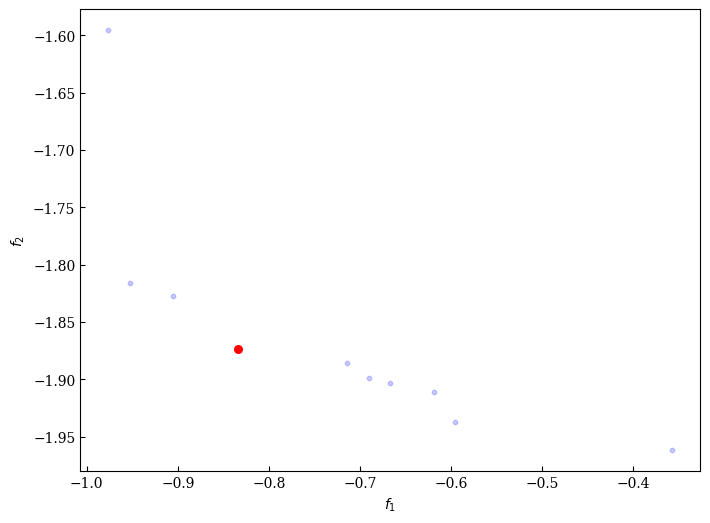
\includegraphics{TargetOptimization_files/figure-pdf/fig-pymoo-parks-output-1.png}

}

\subcaption{\label{fig-pymoo-parks-1}Multi-objective optimization Pareto
front. The selected solution is indicated in red.}

\end{minipage}%
%
\begin{minipage}{0.50\linewidth}

\centering{

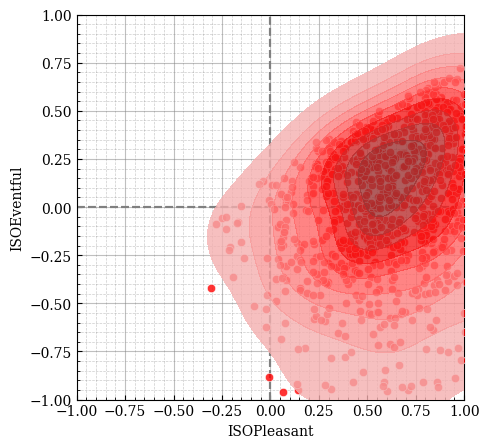
\includegraphics{TargetOptimization_files/figure-pdf/fig-pymoo-parks-output-2.png}

}

\subcaption{\label{fig-pymoo-parks-2}SCM distribution of the derived
target distribution.}

\end{minipage}%

\caption{\label{fig-pymoo-parks}NSGA-II optimization to learn the MSN
parameters which produce the Park ranking.}

\end{figure}%

\begin{Shaded}
\begin{Highlighting}[]
\BuiltInTok{print}\NormalTok{(park\_tgt.summary())}
\end{Highlighting}
\end{Shaded}

\begin{verbatim}
Fitted from direct parameters.
Direct Parameters:
xi:    [0.418 0.284]
omega: [[ 0.164 -0.044]
 [-0.044  0.152]]
alpha: [ 16.628 -30.187]


None
None
\end{verbatim}


  \bibliography{FellowshipRefs.bib}



\end{document}
